\documentclass[11pt,a4paper]{article}
\usepackage[margin=2cm]{geometry}
\usepackage{graphicx}
\usepackage{xcolor}
\usepackage{tcolorbox}
\usepackage{enumitem}
\usepackage{multicol}
\usepackage{amsmath}
\usepackage{amssymb}
\usepackage{fancyhdr}
\usepackage{hyperref}
\usepackage{tikz}
\usetikzlibrary{arrows.meta, positioning, shapes}

% Define colors
\definecolor{mlblue}{RGB}{31, 119, 180}
\definecolor{mlorange}{RGB}{255, 127, 14}
\definecolor{mlgreen}{RGB}{44, 160, 44}
\definecolor{mlred}{RGB}{214, 39, 40}
\definecolor{mlpurple}{RGB}{148, 103, 189}

% Header and footer
\pagestyle{fancy}
\fancyhf{}
\lhead{Week 1: Clustering Workshop}
\rhead{Discovery Worksheet}
\cfoot{Page \thepage}

\title{\Large\textbf{Clustering Discovery Workshop}\\
\vspace{0.5em}
\large In-Class Activity Sheet - Week 1}
\author{BSc Machine Learning for Innovation\\
\textit{Team: \underline{\hspace{5cm}}}}
\date{}

\begin{document}
\maketitle
\thispagestyle{fancy}

\begin{tcolorbox}[colback=mlblue!10, colframe=mlblue!50, title={\textbf{Workshop Objective}}]
Today you'll discover clustering algorithms by building them yourself! Work in teams of 2-3 and document your process as you go.
\end{tcolorbox}

\section*{Activity 1: Manual Clustering Challenge (15 minutes)}

\subsection*{Your Data: Innovation Ideas from a Startup}

Below are 20 innovation ideas plotted by \textbf{Technical Complexity} (x-axis) and \textbf{Market Impact} (y-axis):

\begin{center}
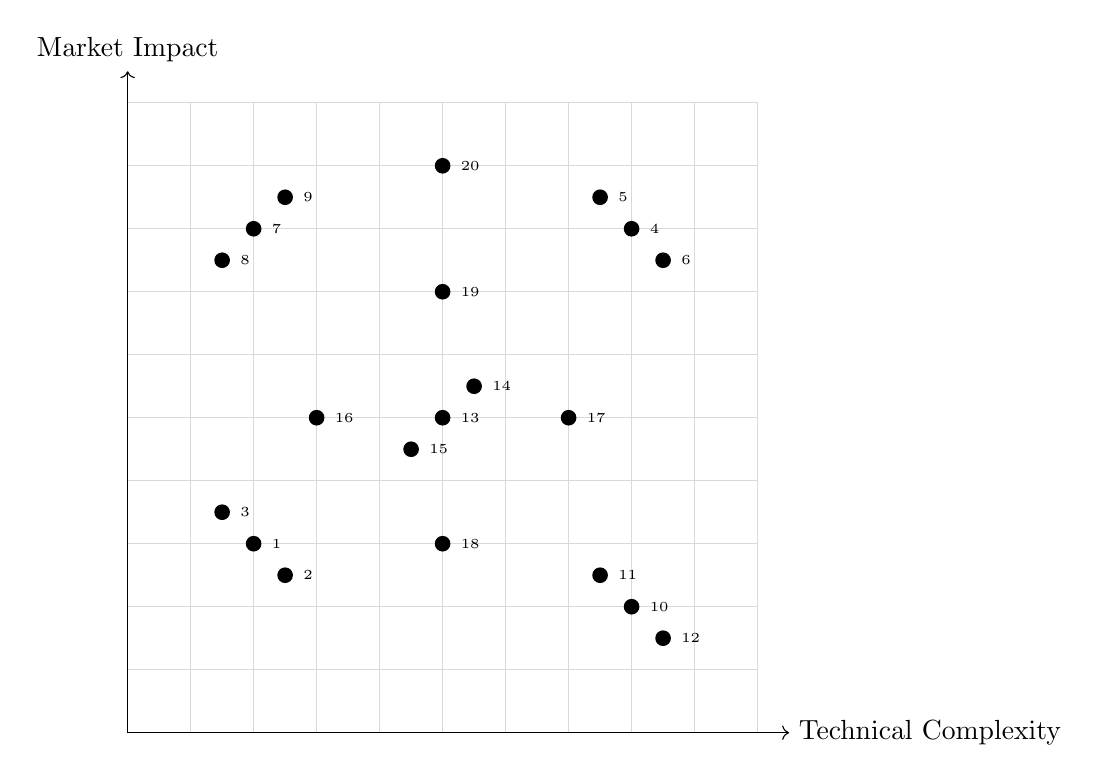
\begin{tikzpicture}[scale=0.8]
% Grid
\draw[gray!30, thin] (0,0) grid (10,10);
\draw[->] (0,0) -- (10.5,0) node[right] {Technical Complexity};
\draw[->] (0,0) -- (0,10.5) node[above] {Market Impact};

% Data points with labels
\node[circle, fill=black, inner sep=2pt, label=right:{\tiny 1}] at (2,3) {};
\node[circle, fill=black, inner sep=2pt, label=right:{\tiny 2}] at (2.5,2.5) {};
\node[circle, fill=black, inner sep=2pt, label=right:{\tiny 3}] at (1.5,3.5) {};
\node[circle, fill=black, inner sep=2pt, label=right:{\tiny 4}] at (8,8) {};
\node[circle, fill=black, inner sep=2pt, label=right:{\tiny 5}] at (7.5,8.5) {};
\node[circle, fill=black, inner sep=2pt, label=right:{\tiny 6}] at (8.5,7.5) {};
\node[circle, fill=black, inner sep=2pt, label=right:{\tiny 7}] at (2,8) {};
\node[circle, fill=black, inner sep=2pt, label=right:{\tiny 8}] at (1.5,7.5) {};
\node[circle, fill=black, inner sep=2pt, label=right:{\tiny 9}] at (2.5,8.5) {};
\node[circle, fill=black, inner sep=2pt, label=right:{\tiny 10}] at (8,2) {};
\node[circle, fill=black, inner sep=2pt, label=right:{\tiny 11}] at (7.5,2.5) {};
\node[circle, fill=black, inner sep=2pt, label=right:{\tiny 12}] at (8.5,1.5) {};
\node[circle, fill=black, inner sep=2pt, label=right:{\tiny 13}] at (5,5) {};
\node[circle, fill=black, inner sep=2pt, label=right:{\tiny 14}] at (5.5,5.5) {};
\node[circle, fill=black, inner sep=2pt, label=right:{\tiny 15}] at (4.5,4.5) {};
\node[circle, fill=black, inner sep=2pt, label=right:{\tiny 16}] at (3,5) {};
\node[circle, fill=black, inner sep=2pt, label=right:{\tiny 17}] at (7,5) {};
\node[circle, fill=black, inner sep=2pt, label=right:{\tiny 18}] at (5,3) {};
\node[circle, fill=black, inner sep=2pt, label=right:{\tiny 19}] at (5,7) {};
\node[circle, fill=black, inner sep=2pt, label=right:{\tiny 20}] at (5,9) {};
\end{tikzpicture}
\end{center}

\subsection*{Task 1: Create Your Clusters}

1. \textbf{Draw circles around groups} you think belong together in the plot above.

2. \textbf{How many clusters did you find?} \underline{\hspace{2cm}}

3. \textbf{Name each cluster} based on its characteristics:
\begin{itemize}
\item Cluster 1: \underline{\hspace{8cm}}
\item Cluster 2: \underline{\hspace{8cm}}
\item Cluster 3: \underline{\hspace{8cm}}
\item Cluster 4: \underline{\hspace{8cm}}
\item Cluster 5: \underline{\hspace{8cm}}
\end{itemize}

4. \textbf{Which ideas don't fit any cluster?} (Outliers): \underline{\hspace{5cm}}

\newpage
\section*{Activity 2: Build K-means Algorithm (20 minutes)}

\subsection*{Step-by-Step K-means Discovery}

You'll now recreate the K-means algorithm using the same data!

\textbf{Round 1: Initial Centers}
\begin{enumerate}
\item Choose K=3 (we want 3 groups)
\item Pick 3 random points as starting centers. Circle them with a different color.
\item Centers chosen: Point \underline{\hspace{1cm}}, Point \underline{\hspace{1cm}}, Point \underline{\hspace{1cm}}
\end{enumerate}

\textbf{Round 2: Assign Points}
\begin{enumerate}
\item For each point, measure distance to all 3 centers
\item Assign each point to its nearest center
\item Color-code your assignments:
\end{enumerate}

\begin{center}
\begin{tabular}{|c|c|c|c|c|}
\hline
Point & Distance to C1 & Distance to C2 & Distance to C3 & Assigned to \\
\hline
1 & & & & \\
\hline
2 & & & & \\
\hline
3 & & & & \\
\hline
... & ... & ... & ... & ... \\
\hline
\end{tabular}
\end{center}

\textbf{Round 3: Update Centers}
\begin{enumerate}
\item Calculate the average position of all points in each cluster
\item New Center 1: (\underline{\hspace{1cm}}, \underline{\hspace{1cm}})
\item New Center 2: (\underline{\hspace{1cm}}, \underline{\hspace{1cm}})
\item New Center 3: (\underline{\hspace{1cm}}, \underline{\hspace{1cm}})
\end{enumerate}

\textbf{Round 4: Check Convergence}
\begin{itemize}
\item Did any points change clusters? YES / NO
\item If YES, repeat Round 2-3
\item If NO, you're done!
\end{itemize}

\begin{tcolorbox}[colback=mlgreen!10, colframe=mlgreen!50, title={\textbf{Discovery Question}}]
How is your K-means result different from your manual clustering? Why?
\vspace{3cm}
\end{tcolorbox}

\newpage
\section*{Activity 3: Distance Metrics Exploration (15 minutes)}

\subsection*{Different Ways to Measure ``Close''}

Consider these two innovation profiles:
\begin{itemize}
\item \textbf{Idea A}: Tech=8, Impact=3, Cost=5
\item \textbf{Idea B}: Tech=5, Impact=7, Cost=6
\end{itemize}

\subsection*{Calculate Different Distances:}

\textbf{1. Euclidean Distance} (straight line):
$$d = \sqrt{(8-5)^2 + (3-7)^2 + (5-6)^2} = \sqrt{\underline{\hspace{1cm}} + \underline{\hspace{1cm}} + \underline{\hspace{1cm}}} = \underline{\hspace{2cm}}$$

\textbf{2. Manhattan Distance} (city blocks):
$$d = |8-5| + |3-7| + |5-6| = \underline{\hspace{1cm}} + \underline{\hspace{1cm}} + \underline{\hspace{1cm}} = \underline{\hspace{2cm}}$$

\textbf{3. Maximum Distance} (biggest difference):
$$d = \max(|8-5|, |3-7|, |5-6|) = \max(\underline{\hspace{1cm}}, \underline{\hspace{1cm}}, \underline{\hspace{1cm}}) = \underline{\hspace{2cm}}$$

\begin{tcolorbox}[colback=mlorange!10, colframe=mlorange!50, title={\textbf{Innovation Insight}}]
Which distance metric would you use for:
\begin{itemize}
\item Finding similar products for customers? \underline{\hspace{5cm}}
\item Grouping projects by resource needs? \underline{\hspace{5cm}}
\item Identifying competing innovations? \underline{\hspace{5cm}}
\end{itemize}
\end{tcolorbox}

\section*{Activity 4: Cluster Quality Assessment (10 minutes)}

\subsection*{How Good Are Your Clusters?}

Rate your clusters on these criteria (1-5 scale):

\begin{center}
\begin{tabular}{|l|c|p{6cm}|}
\hline
\textbf{Criterion} & \textbf{Score (1-5)} & \textbf{Why?} \\
\hline
\textbf{Cohesion} & & \\
Points in same cluster are similar & & \\
\hline
\textbf{Separation} & & \\
Different clusters are distinct & & \\
\hline
\textbf{Coverage} & & \\
Most points belong to a cluster & & \\
\hline
\textbf{Balance} & & \\
Clusters have similar sizes & & \\
\hline
\textbf{Interpretability} & & \\
Clusters make business sense & & \\
\hline
\end{tabular}
\end{center}

\textbf{Overall Quality Score}: \underline{\hspace{2cm}} / 25

\newpage
\section*{Activity 5: Innovation Application (15 minutes)}

\subsection*{From Clusters to Strategy}

Based on your clustering results, create an innovation strategy:

\textbf{1. Priority Matrix}

Place your clusters in the appropriate quadrant:

\begin{center}
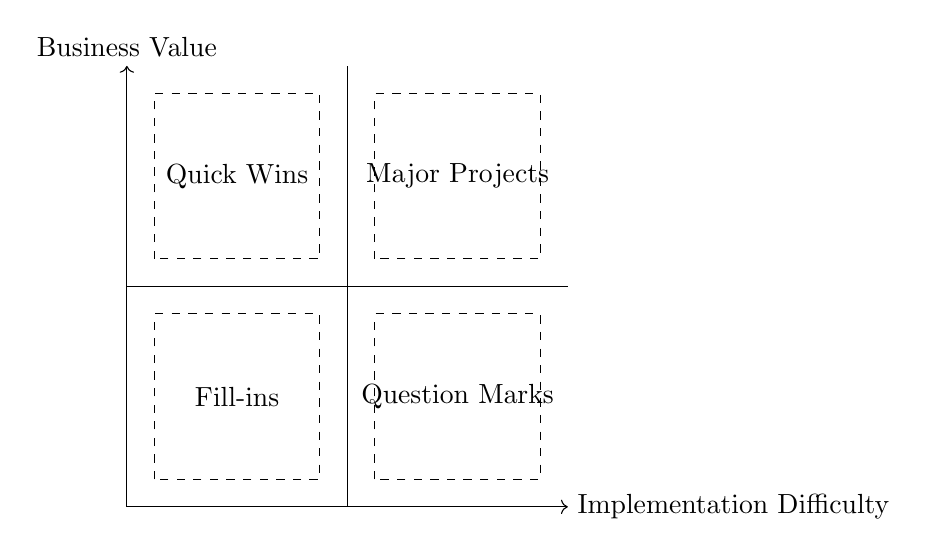
\begin{tikzpicture}[scale=0.7]
\draw[->] (0,0) -- (8,0) node[right] {Implementation Difficulty};
\draw[->] (0,0) -- (0,8) node[above] {Business Value};
\draw (0,4) -- (8,4);
\draw (4,0) -- (4,8);

\node at (2,6) {Quick Wins};
\node at (6,6) {Major Projects};
\node at (2,2) {Fill-ins};
\node at (6,2) {Question Marks};

% Areas for clusters
\draw[dashed] (0.5,4.5) rectangle (3.5,7.5);
\draw[dashed] (4.5,4.5) rectangle (7.5,7.5);
\draw[dashed] (0.5,0.5) rectangle (3.5,3.5);
\draw[dashed] (4.5,0.5) rectangle (7.5,3.5);
\end{tikzpicture}
\end{center}

\textbf{2. Resource Allocation}

How would you allocate 100 points of resources?
\begin{itemize}
\item Cluster 1: \underline{\hspace{2cm}} points
\item Cluster 2: \underline{\hspace{2cm}} points
\item Cluster 3: \underline{\hspace{2cm}} points
\item Outliers/Other: \underline{\hspace{2cm}} points
\end{itemize}

\textbf{3. Innovation Roadmap}

Order your clusters for implementation:
\begin{enumerate}
\item First: \underline{\hspace{8cm}}
\item Second: \underline{\hspace{8cm}}
\item Third: \underline{\hspace{8cm}}
\end{enumerate}

\section*{Reflection \& Synthesis (5 minutes)}

\begin{tcolorbox}[colback=mlpurple!10, colframe=mlpurple!50, title={\textbf{Key Discoveries}}]
\textbf{1. What surprised you about clustering?}
\vspace{2cm}

\textbf{2. How would clustering help your organization?}
\vspace{2cm}

\textbf{3. What challenges did you encounter?}
\vspace{2cm}
\end{tcolorbox}

\textbf{Team Members:}
\begin{itemize}
\item \underline{\hspace{8cm}}
\item \underline{\hspace{8cm}}
\item \underline{\hspace{8cm}}
\end{itemize}

\end{document}